% to compile:
% bibtex project
% bibtex project
% pdflatex project

\documentclass[11pt]{article}
\usepackage{graphicx}
\usepackage{pdflscape}
\usepackage{amssymb}
\PassOptionsToPackage{hyphens}{url}\usepackage{hyperref}
\usepackage{listings}
\lstset{
basicstyle=\small\ttfamily,
columns=flexible,
breaklines=true
}
\usepackage{graphicx}
\graphicspath{ {./images/} }

\title{A Domain-Specific Knowledge Graph for News Item Recommendations and Information Retrieval}
\author{Author: Christopher Eaves-Kohlbrenner \\ Supervisor: Michael Zakharyaschev}

\begin{document}
\maketitle

\begin{center}
\hfill \break
\hfill \break
\hfill \break
MSc Data Science project\\
Department of Computer Science and Information Systems\\
Birkbeck College, University of London\\
2021\\
\hfill \break
\hfill \break
\hfill \break

\textit{This report is substantially the result of my own work, expressed in my own words, except where explicitly indicated in the text. I have read and understood the sections on plagiarism in the Programme Handbook and the College web site. I give my permission for it to be submitted to the JISC Plagiarism Detection Service. \\
\hfill \break
The report may be freely copied and distributed provided the source is explicitly acknowledged.}
\end{center}

% \end{center}

\newpage
\begin{abstract}
TBD...
\end{abstract}

\newpage
\tableofcontents

\newpage
\section{Glossary}
\begin{itemize}
\item KG - Knowledge graph
\item ML - Machine learning
\item NewsML\footnote{\url{https://iptc.org/standards/newsml-g2/}} - XML format for news items and metadata
\item NER - Named entity recognition
\item NLP - Natural language processing
\item OWL - Web Ontology Language
\item SRL - Statistical relational learning
\item ST - Semantic technology
\item XML - Extensible Markup Language format for encoding documents
\end{itemize}

\newpage
\section{Introduction}
TODO: repurpose some proposal sections... and wait until the rest of the research/paper is done, so I can introduce and briefly summarize here.

\subsection{Problem}
Problem...
\subsection{Project Objectives}
Project Objectives...
\subsection{Summary of Findings}
Summary of Findings...
\subsection{Report Outline}
Report Outline...
\subsection{Technical Specifications}
Technical Specifications...

\section{Context and Background}
TODO: repurpose some proposal sections...
\subsection{Knowledge Graphs}
\subsection{Network stuff?}
similar to "A graph neural network path to network centralities.pdf"?
% https://www.dcs.bbk.ac.uk/r/studentprojects/exampleprojects/msc/



\section{Data}
A substantial corpus of text data was required in order to apply semantic, natural language, and knowledge graph techniques in this analysis.

In the media space, Reuters has produced high-quality journalism since 1851 and has contributed to the data science domain via datasets like Reuters-21578\cite{reuters-21578}, RCV1\cite{lewis2004rcv1}, and others\cite{reuters-corpora} being made available for natural language processing, information retrieval, and machine learning research\footnote{\url{https://trec.nist.gov/data/reuters/reuters.html}}.

\subsection{Data Set Collection}
This analysis focuses on the ``Reuters News Archive (30 Days)" data set, provided by Reuters as a ``full corpus of English articles"\footnote{\url{https://aws.amazon.com/marketplace/pp/prodview-qwmkdffmmjesa}}.

A few key attributes of this data set include the following, which make it suitable for this analysis:
\begin{itemize}
  \item{This is English language text data. No other languages are included, which eliminates any challenges around multilingual NLP.}
  \item{The corpus covers various areas including breaking financial and general news and global coverage of politics, sports, entertainment, and technology. This enables a broad cross-section of information in different areas to be represented in a knowledge graph.}
  \item{The data set spans 30 days of news from 1-30 September 2019, which means the knowledge graph will be time-bound to this 30-day period.}
  \item{The data set includes 59,542 news items in XML format, a sufficient volume of data to populate a media knowledge graph.}
  \item{The XML documents follow the NewsMLG2 standard\footnote{\url{https://iptc.org/standards/newsml-g2/}}, a media industry standard of structuring news metadata for semantic technology.}
\end{itemize}

As an example, a sample XML document is available in \hyperref[sec:AppendixXML]{``Appendix XML"}. The analysis below describes how the XML properties are extracted and ingested into a graph database format to build the knowledge graph.

\subsection{Data Input and Preprocessing}
Creating a knowledge graph requires a transformation of the news data from its original, semi-structured XML document form into a structured format. This was a multi-step process.

  \subsubsection{Source data}
  The first step was to download the XML documents from AWS S3 into a local directory. As a one-time step, this was done manually via the AWS S3 user interface.

  \subsubsection{Extract XML properties (\lstinline{item_xml_docs_to_csv.py})}
  Next a batched job converted the directory of local XML documents into CSV format, with a CSV for each 10,000 items and a row for each of the 59,542 news items. This job output six CSV files with columns for XML filename, datetime, guid, slugline, headline, description, genres, subjects, bodyLengthChars, and bodyLengthWords (see \hyperref[sec:AppendixA]{``Appendix A"}).
  
  \subsubsection{Ontology development and linked data (\lstinline{wikidata_to_wikipedia_url.py})}
  A manual step categorised the 415 subjects extracted from the news item XML documents, subjects (e.g., Aquatic Sports, United Kingdom, Middle East, and Books) into categories (e.g., sport, country, region, art and culture). Next a script mapped each subject to a Wikidata ID and Wikipedia URL, to enable linked data with Wikidata.
  
  \subsubsection{Data cleaning (\lstinline{data-dimensions.ipynb})}
  The resulting CSVs of enriched subjects, news items, and genres were read into a Pandas dataframe using a Jupyter notebook. This Jupyter notebook yields helpful insights:
  \begin{itemize}
    \item{It gives a sense of the overall shape of the text data, calling attention to outliers with very long or nonexistent text bodies and expected word counts (see \textit{Figure 1}).}

    \item{It illustrates the power-law distribution of subjects. For example, seven\footnote{Americas, North America, Europe, United States, Emerging Market Countries, Asia / Pacific, Western Europe, Asia} of 415 subjects (1.7\%) are present on more than 25\% of news items, but 329 out of 414 subjects (79.5\%) are present on less than 1\% of news items (see \textit{Figure 2} and \textit{Figure 3}).

    \begin{table}
      \begin{tabular}{ |p{1cm}|p{2.25cm}|p{2.25cm}|p{2.25cm}|p{2.25cm}|  }
      \hline
      \multicolumn{5}{|c|}{NewsItem dataframe (\lstinline{df.describe()})} \\
      \hline
      &Character length&Non-whitespace character length&Word count&Average word length\\
      \hline
      count&59542&59542&59542&59542\\
      mean&2759.12&2201.52&326.52&7.59\\
      std&7472.39&6149.59&960.27&1.38\\
      min&0&0&1&0\\
      25\%&482&380&44&6.64\\
      50\%&959&761&106&7.20\\
      75\%&2952&2346&356&8.45\\
      max&294233&251216&42360&43.57\\
      \hline
      \end{tabular}
      \caption{\textit{NewsItem dataframe}}
    \end{table}

    \begin{figure}
      \centerline{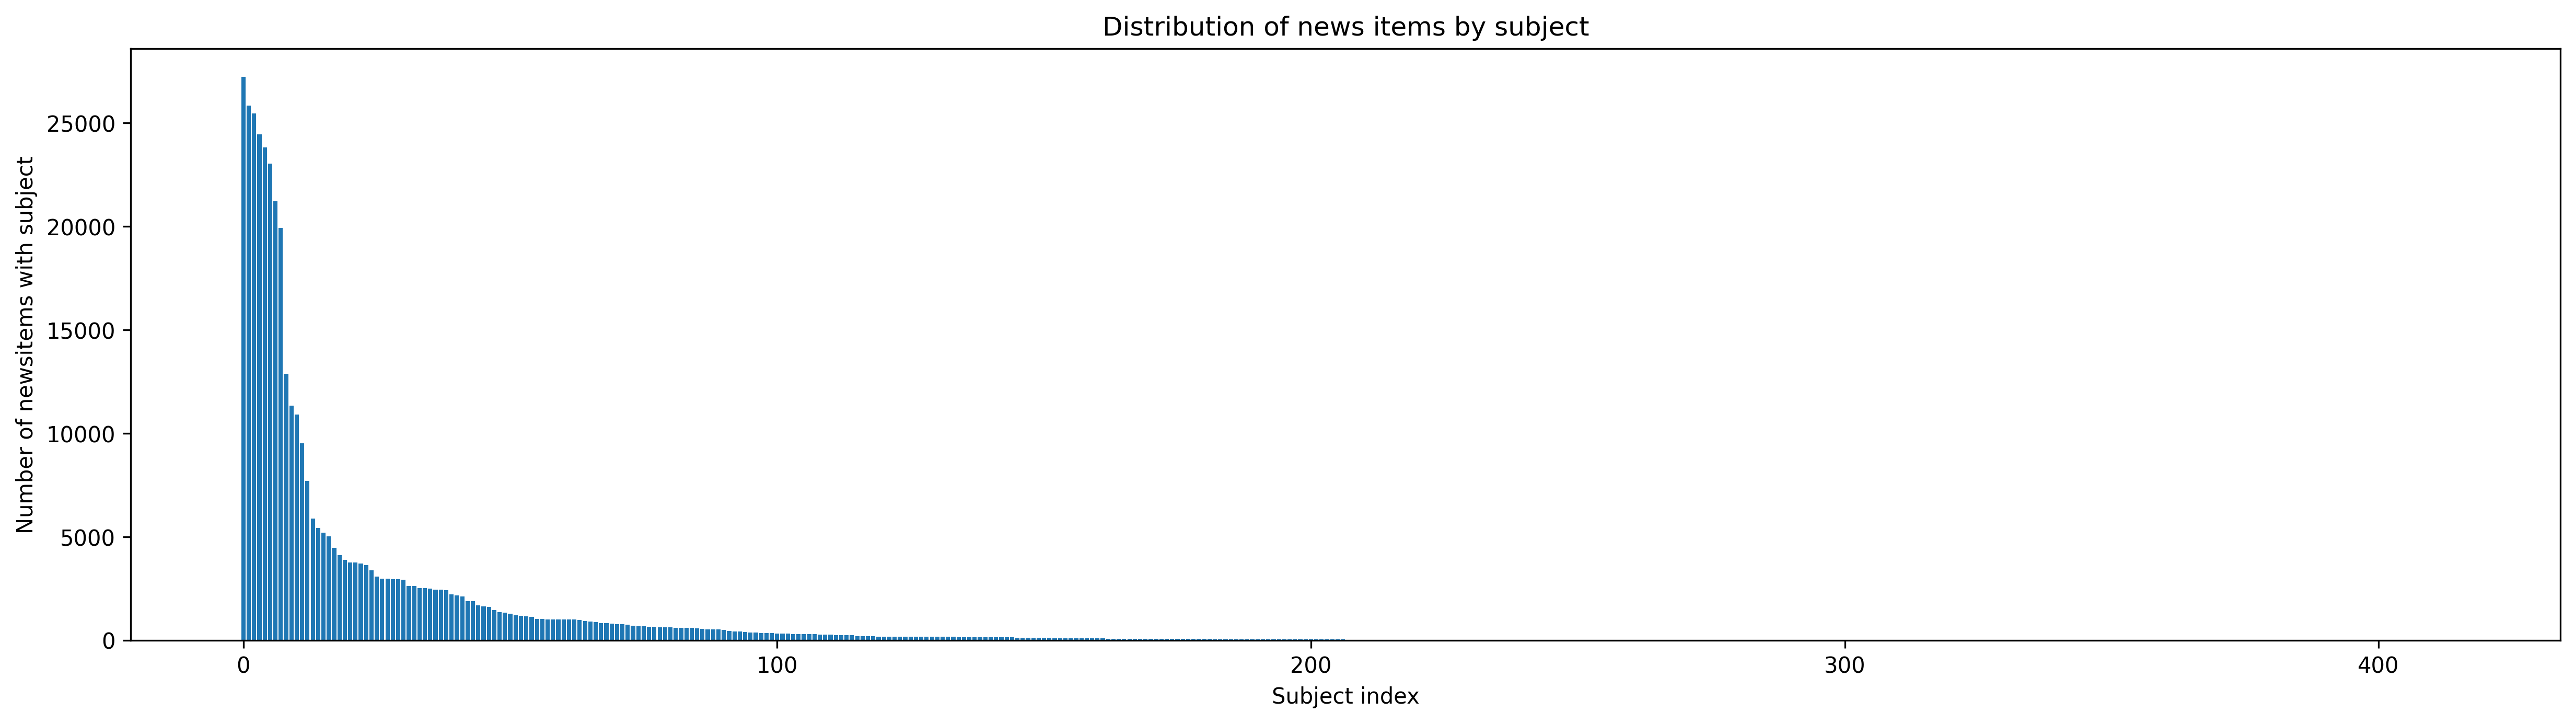
\includegraphics[scale=0.35]{distribution_news_item_subject}}
      \caption{\textit{Distribution of news items by subject}}
    \end{figure}

    \begin{figure}
      \centerline{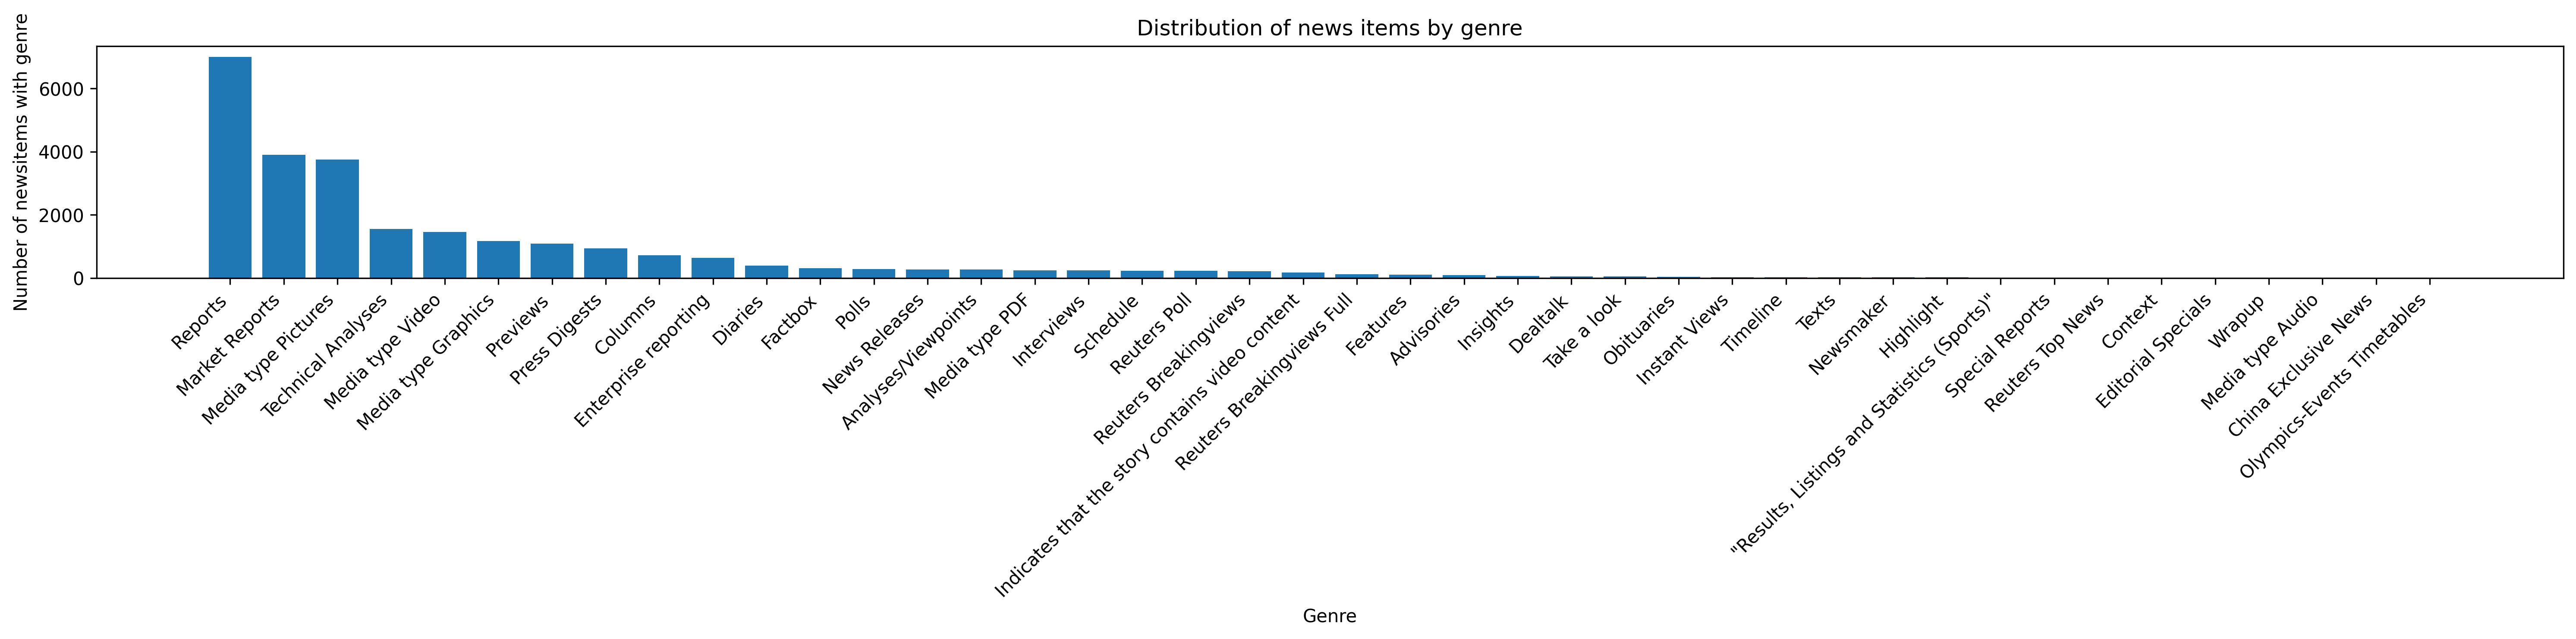
\includegraphics[scale=0.3]{distribution_news_item_genre}}
      \caption{\textit{Distribution of news items by genre}}
    \end{figure}

    }
  \end{itemize}
  (see\hyperref[sec:AppendixB]{``Appendix B"})
  
  \subsubsection{Data challenges}
  Cleaning this dataset presented a few unique challenges, which will be considered in the NLP section below.
  \begin{itemize}
    \item{This corpus included some XML documents with unique encoding issues between UTF-8 encoding and plain text. For example, some of the XML documents\footnote{tag:reuters.com,2019:newsml\_CqtHM2P1a} included Tweets with emojis. A future effort could handle such emojis more gracefully. Furthermore, some apostrophes were transformed \footnote{For example, headline ``BREAKINGVIEWS-Carmakers,\"A\^o antitrust probe is more smoke than fire" (tag:reuters.com,2019:newsml\_L2N25X0YW).}
    }
    \item{Some documents include table-formatted text, with many spaces meant to be rendered in a monospace format. In this case, a simple logic to consider a single space as a word boundary is not correct.\footnote{For example, item tag:reuters.com,2019:newsml\_L3N2602HC:991614233 should not be considered to have 76,783 words, despite having 294,233 spaces when counting all whitespace.}}
    \item{Some documents are incredibly long direct quotations transcribed from an event. These should be handled differently than other news reports.\footnote{For example, item tag:reuters.com,2019:newsml\_CqtYP8GSa:1548902168.XML is a full transcript of a committee hearing on US-China relations.}}
  \end{itemize}

  \subsubsection{Graph database ingestion (\lstinline{csvs_to_neo4j.cypher})}
  Finally, Cypher queries were run to ingest the primary metadata from each cleaned XML news item into Neo4j as a property graph with initial relationships (see\hyperref[sec:AppendixC]{``Appendix C"}). After running these Cypher queries, a prototype knowledge graph is available for meaningful queries and initial information retrieval (see\hyperref[sec:DataSetEvaluation]{``Data Set Evaluation"} below). This step uses Neo4j, Cypher, and APOC to load the cleaned CSV, create Neo4j nodes for each NewsItem, Subject, and Genre, add properties to the nodes, and create \lstinline{-[:HAS_GENRE]->} and \lstinline{-[:HAS_SUBJECT]->} relationships.



\subsection{Data Set Evaluation}
\label{sec:DataSetEvaluation}

With the data sourcing, cleaning, and graph database ingestion complete, we can evaluate the raw data and begin to see the practical value of a knowledge graph in terms of information retrieval.

At a basic level, the overall shape of the data and graph become clear. As shown in \textit{Table 2} and \textit{Table 3}, nearly 60,000 nodes are now available in the Neo4j graph database. Furthermore, there is interesting variance in the number of relationships per node, while keeping the properties per node constant across all NewsItems, Genres, and Subjects.


\begin{table}
  \begin{tabular}{ |p{3cm}||p{2cm}|p{7cm}|  }
  \hline
  \multicolumn{3}{|c|}{Neo4j Knowledge Graph Nodes: high-level view of graph DB schema} \\
  \hline
  Node (Label)& Count &Properties\\
  \hline
  NewsItem&59,542&guid, filename, headline, slugline, datetime, genres, bodyLengthWords, subjects, description, bodyLengthChars, bodyLengthCharsNonWhitespace\\
  \hline
  Subject&414&category, subject, wikidataURL, wikipediaURL\\
  \hline
  Genre&42&genre\\
  \hline
  \end{tabular}
  \caption{\textit{Initial Knowledge Graph overview}}
\end{table}

\begin{table}
  \begin{lstlisting}
  MATCH (n)
  WITH labels(n) as labels, size(keys(n)) as props, size((n)--()) as degree
  RETURN
  DISTINCT labels,
  count(*) AS NumNodes,
  avg(props) AS AvgNumPropPerNode,
  min(props) AS MinNumPropPerNode,
  max(props) AS MaxNumPropPerNode,
  avg(degree) AS AvgNumRelationships,
  min(degree) AS MinNumRelationships,
  max(degree) AS MaxNumRelationships
  \end{lstlisting}

  \begin{tabular}{ |p{2cm}|p{1cm}|p{1.5cm}|p{1.5cm}|p{1.5cm}|p{1.5cm}|p{1.5cm}|p{1.5cm}| }
  \hline
  labels&Num-Nodes&AvgNum-PropPer-Node&MinNum-PropPer-Node&MaxNum-PropPer-Node&AvgNum-Relation-ships&MinNum-Relation-ships&MaxNum-Relation-ships\\
  \hline
  [``NewsItem"]&59542&11&11&11&7.55&0&94\\
  \hline
  [``Genre"]&42&1&1&1&618.31&1&7250\\
  \hline
  [``Subject"]&415&5&5&5&1021.13&0&27250\\
  \hline
  \end{tabular}

  \caption{\textit{Cypher query\protect \footnotemark to inventory initial nodes and relationships in the knowledge graph}}
\end{table}

\footnotetext{\url{https://neo4j.com/developer/kb/how-do-i-produce-an-inventory-of-statistics-on-nodes-relationships-properties/}}


More significantly, at this point the knowledge graph's practical value begins to become evident, as some human-interpretable queries are now possible, which were not originally possible with the raw data. Whereas the unstructured collection of semi-structured XML documents could not be queried, now we can present meaningful queries over the dataset, including the following\footnote{some of these are available in \lstinline{query_ky.cypher}...potentially to include in Appendix}:

\begin{itemize}
  \item{Finding all news items that have two specific subjects or all items that have more than a certain number of genre or subject relationships (see \textit{Figure 3}).}
  \item{Finding the shortest news items and longest news items by length in characters (see \textit{Figure 4}).}
  \item{Finding the subjects and genres assigned to the most items (see \textit{Figure 5}). Note that these figures confirm what was already discovered in the distribution findings of \textit{Figure 1} and \textit{Figure 2}.}
  \item{Finding the shortest path between two items, perhaps to quickly see what some news stories have in common (see \textit{Figure 6}).}
\end{itemize}


\begin{figure}
  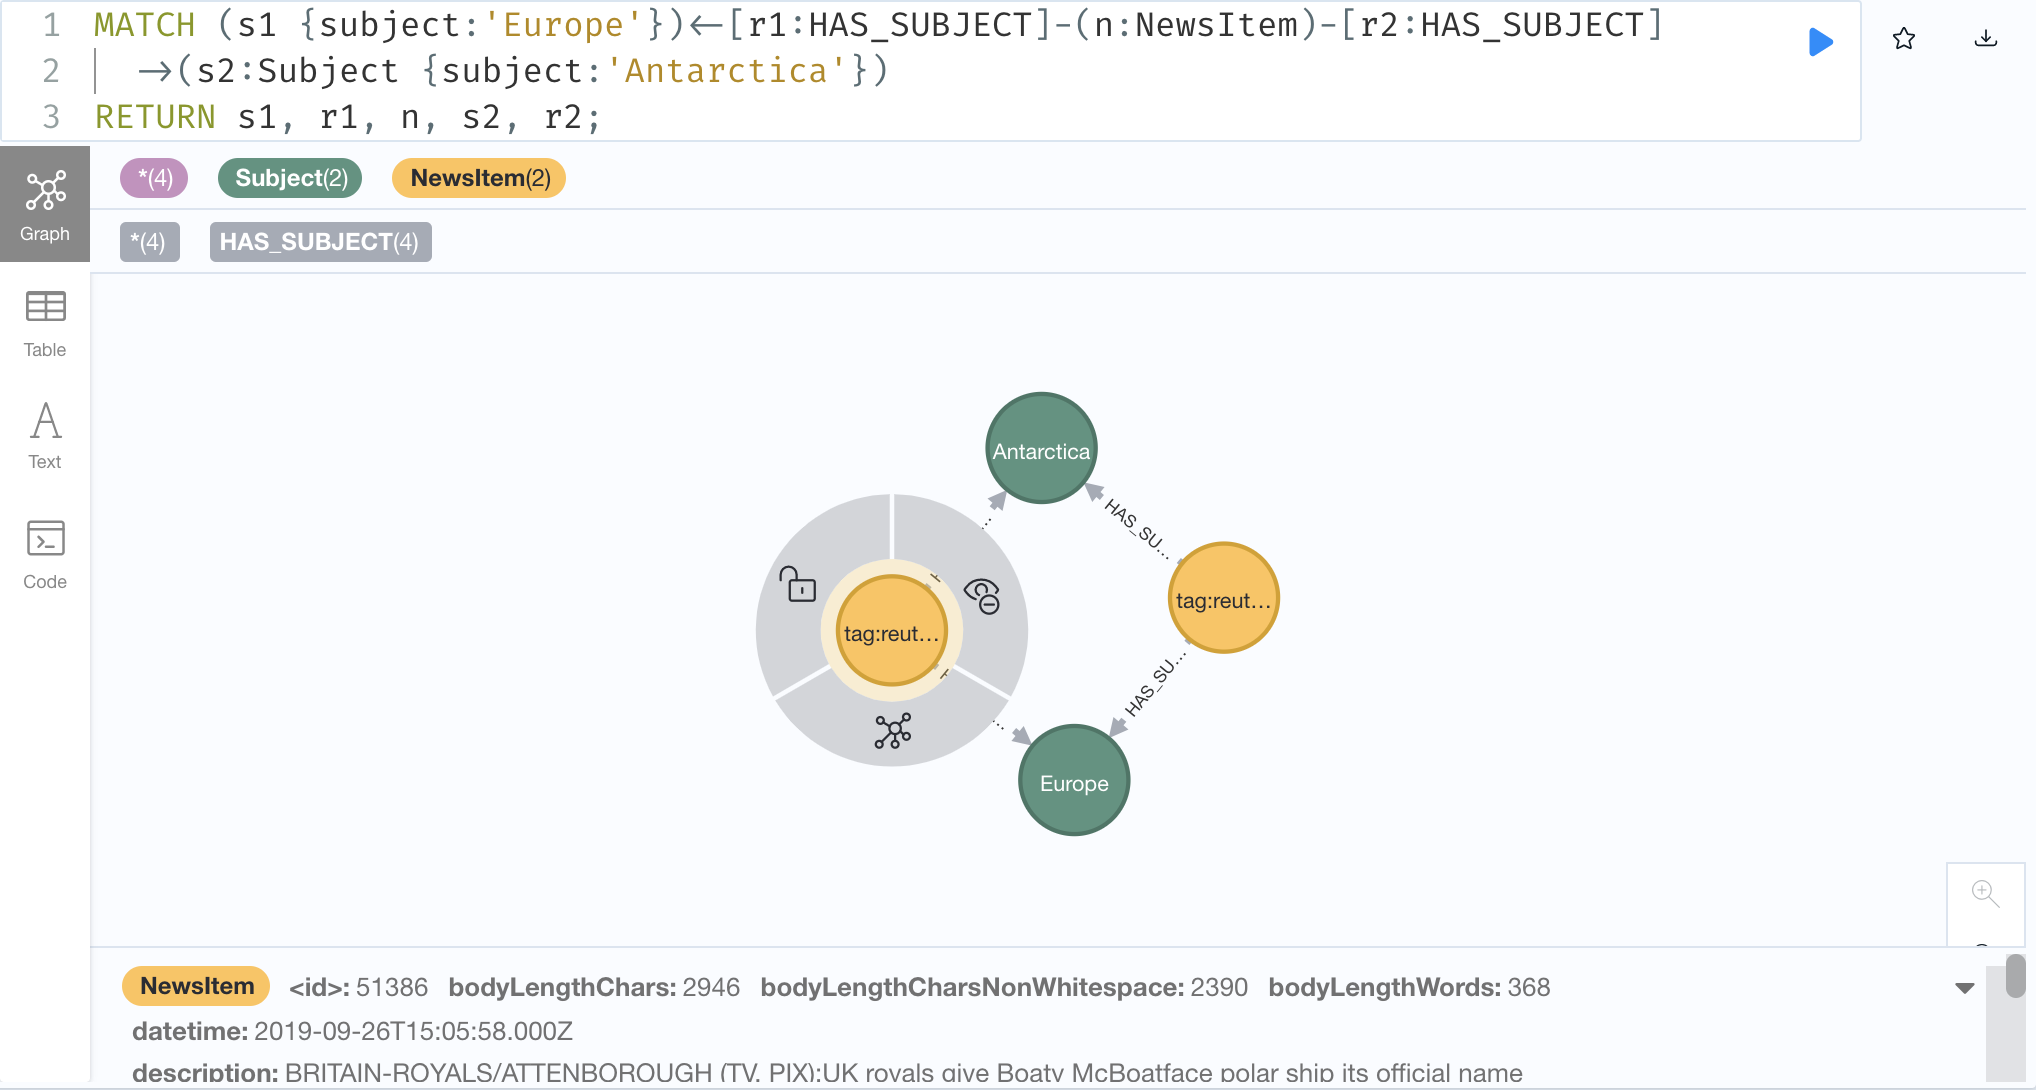
\includegraphics[scale=0.2]{00-news-items-antarctica-europe}
  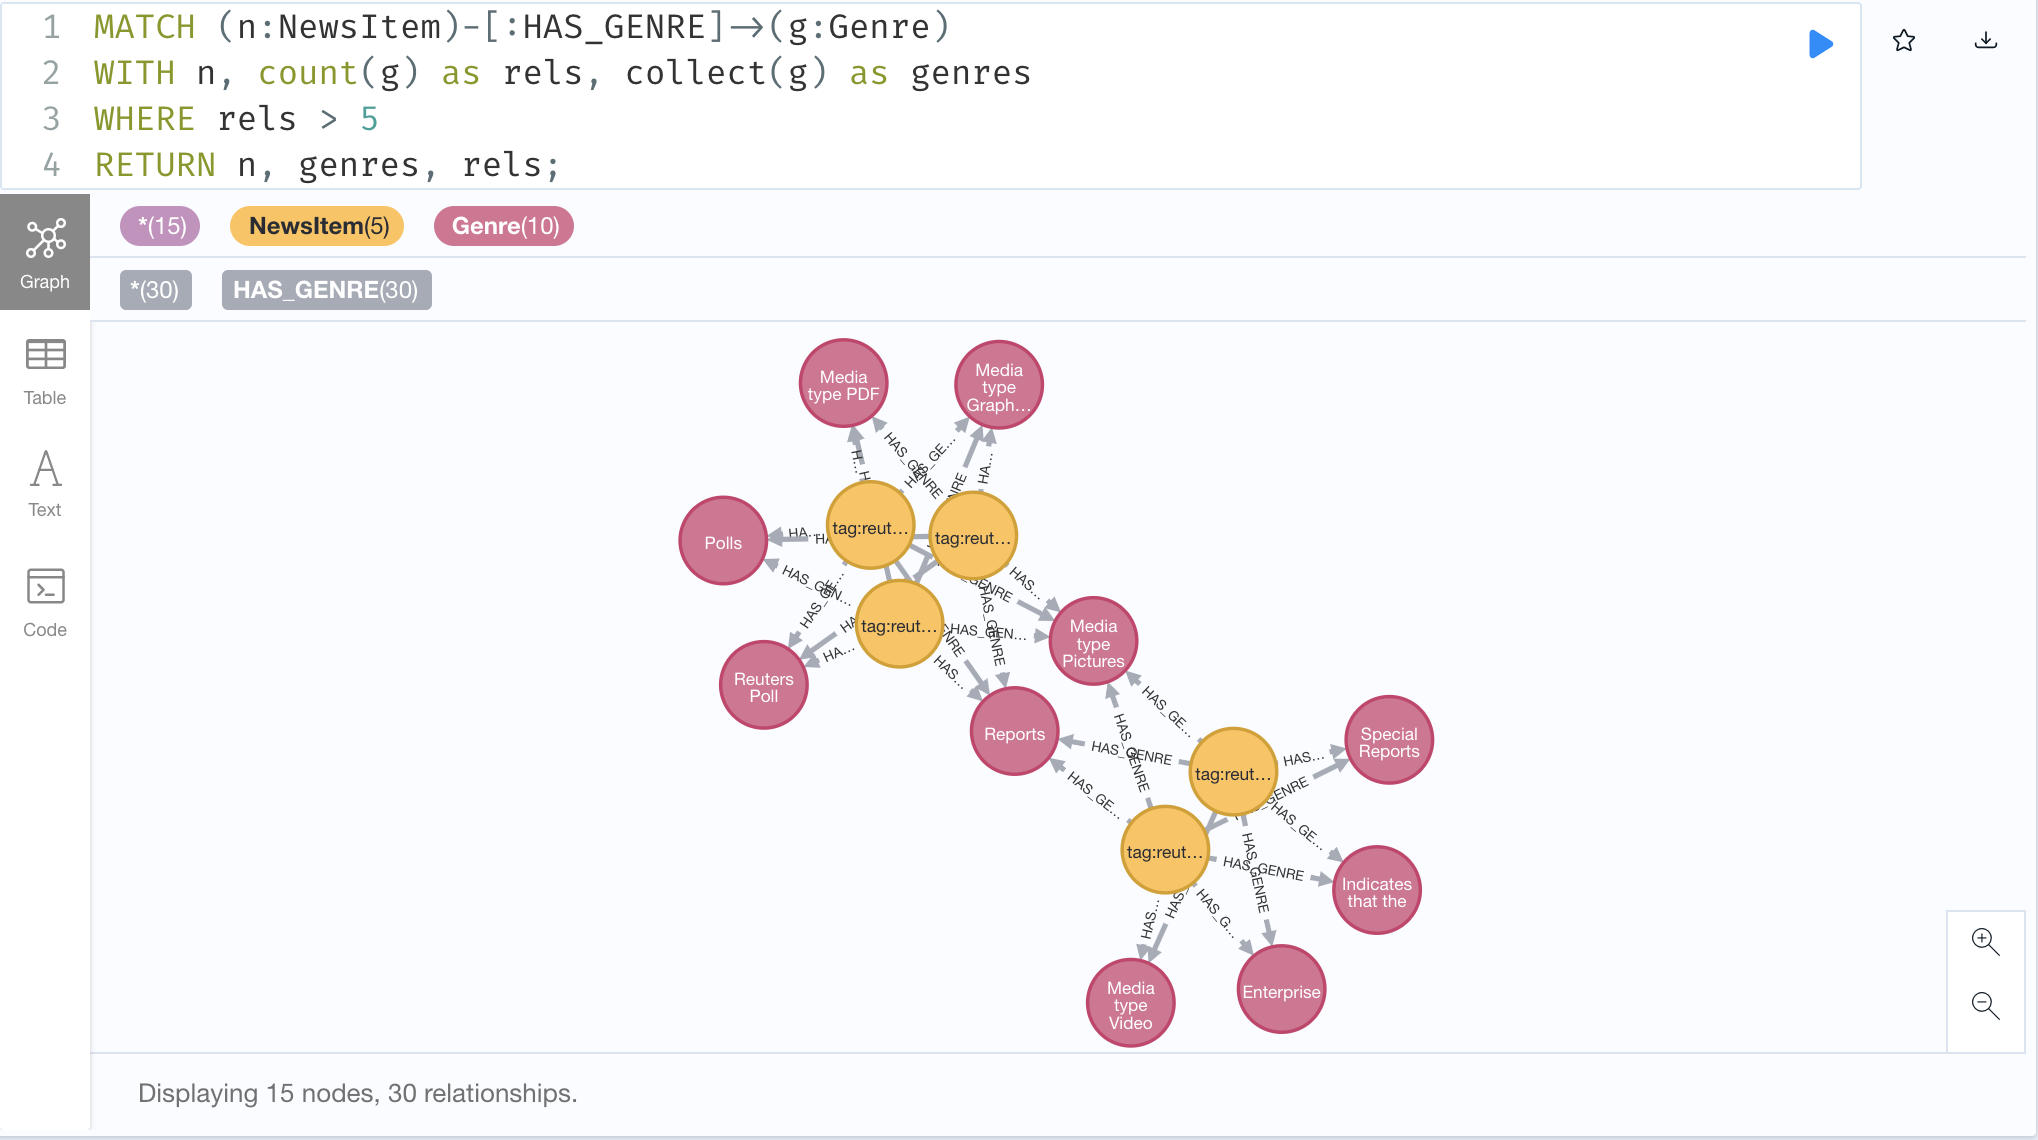
\includegraphics[scale=0.2]{00-news-items-more-than-five-genres}
  \caption{\textit{Knowledge graph Cypher queries: subject and genre relationships)}}
\end{figure}

\begin{figure}
  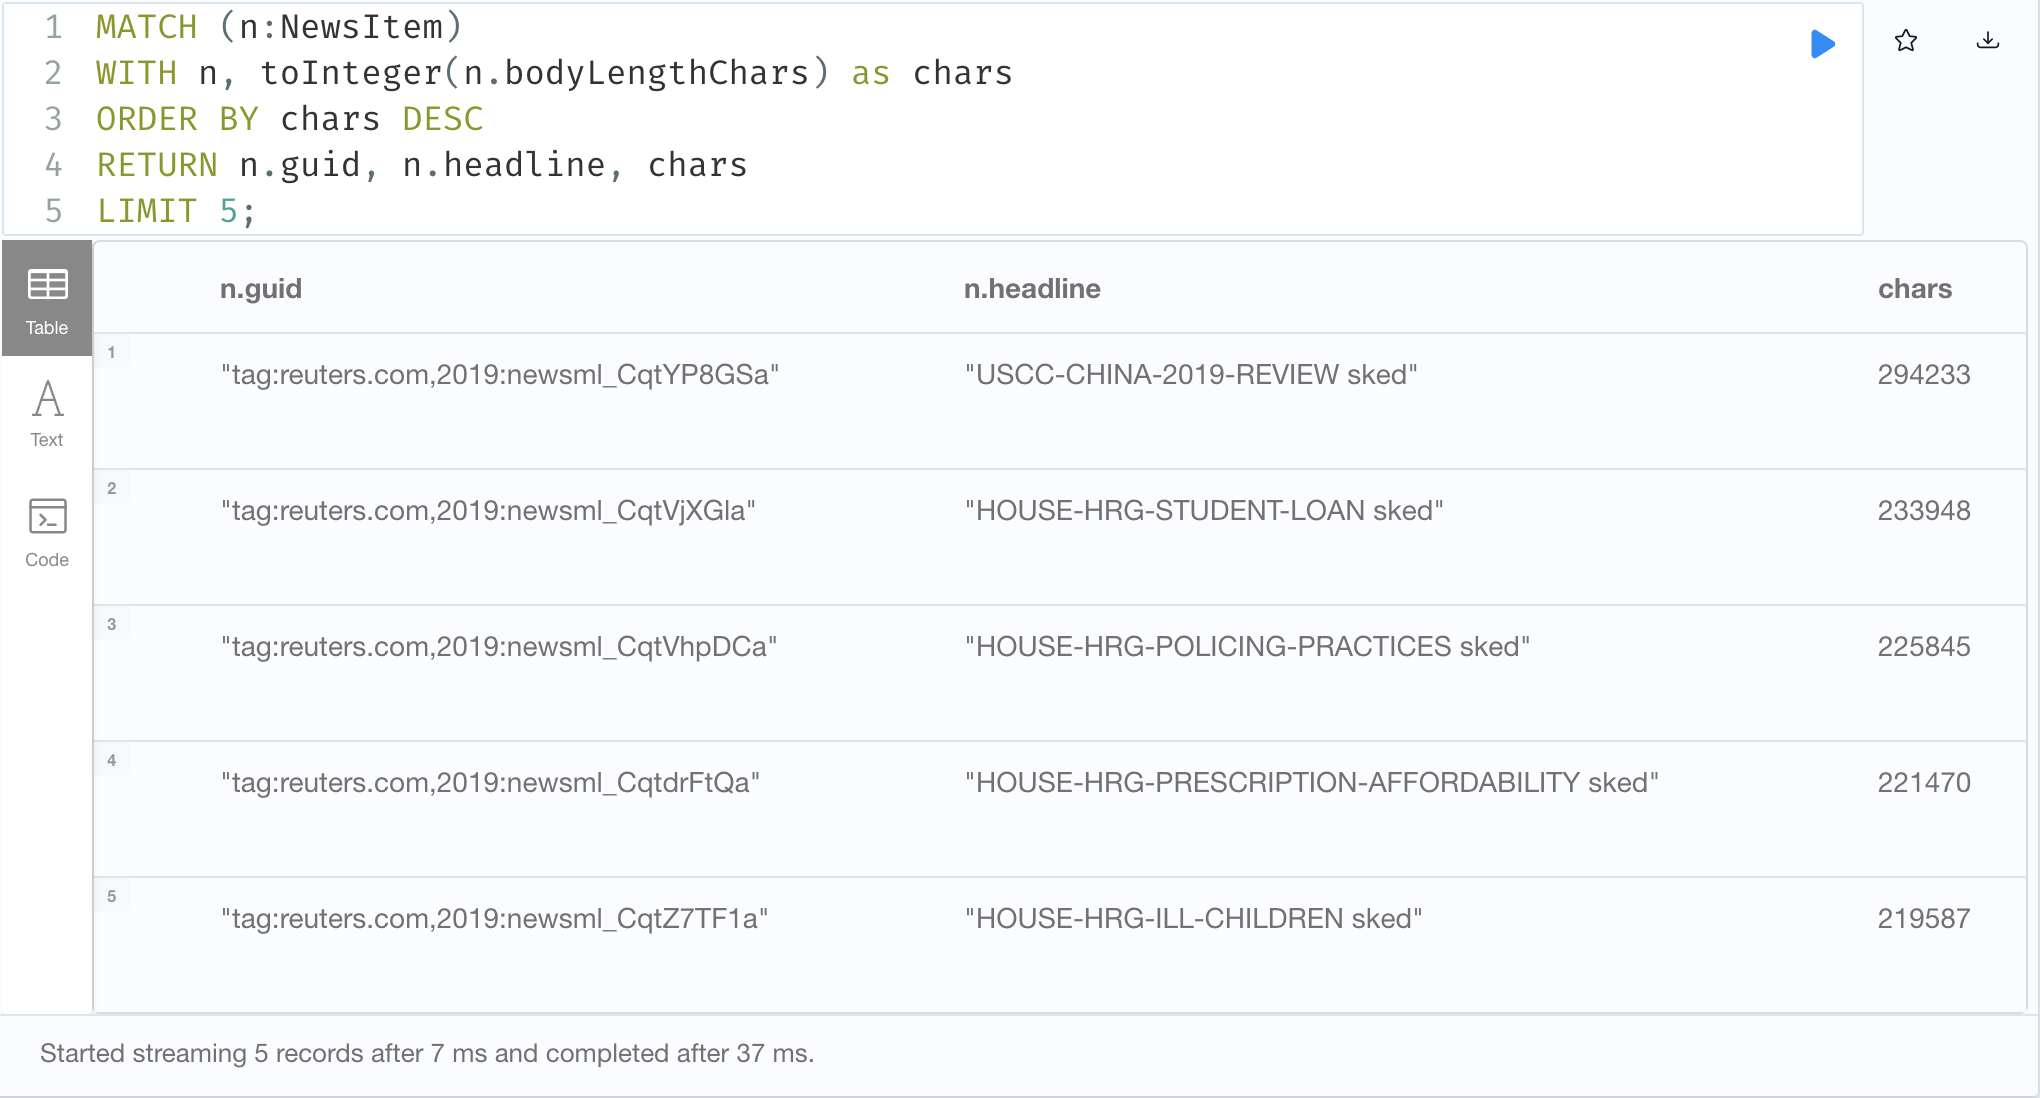
\includegraphics[scale=0.2]{01-longest-items}
  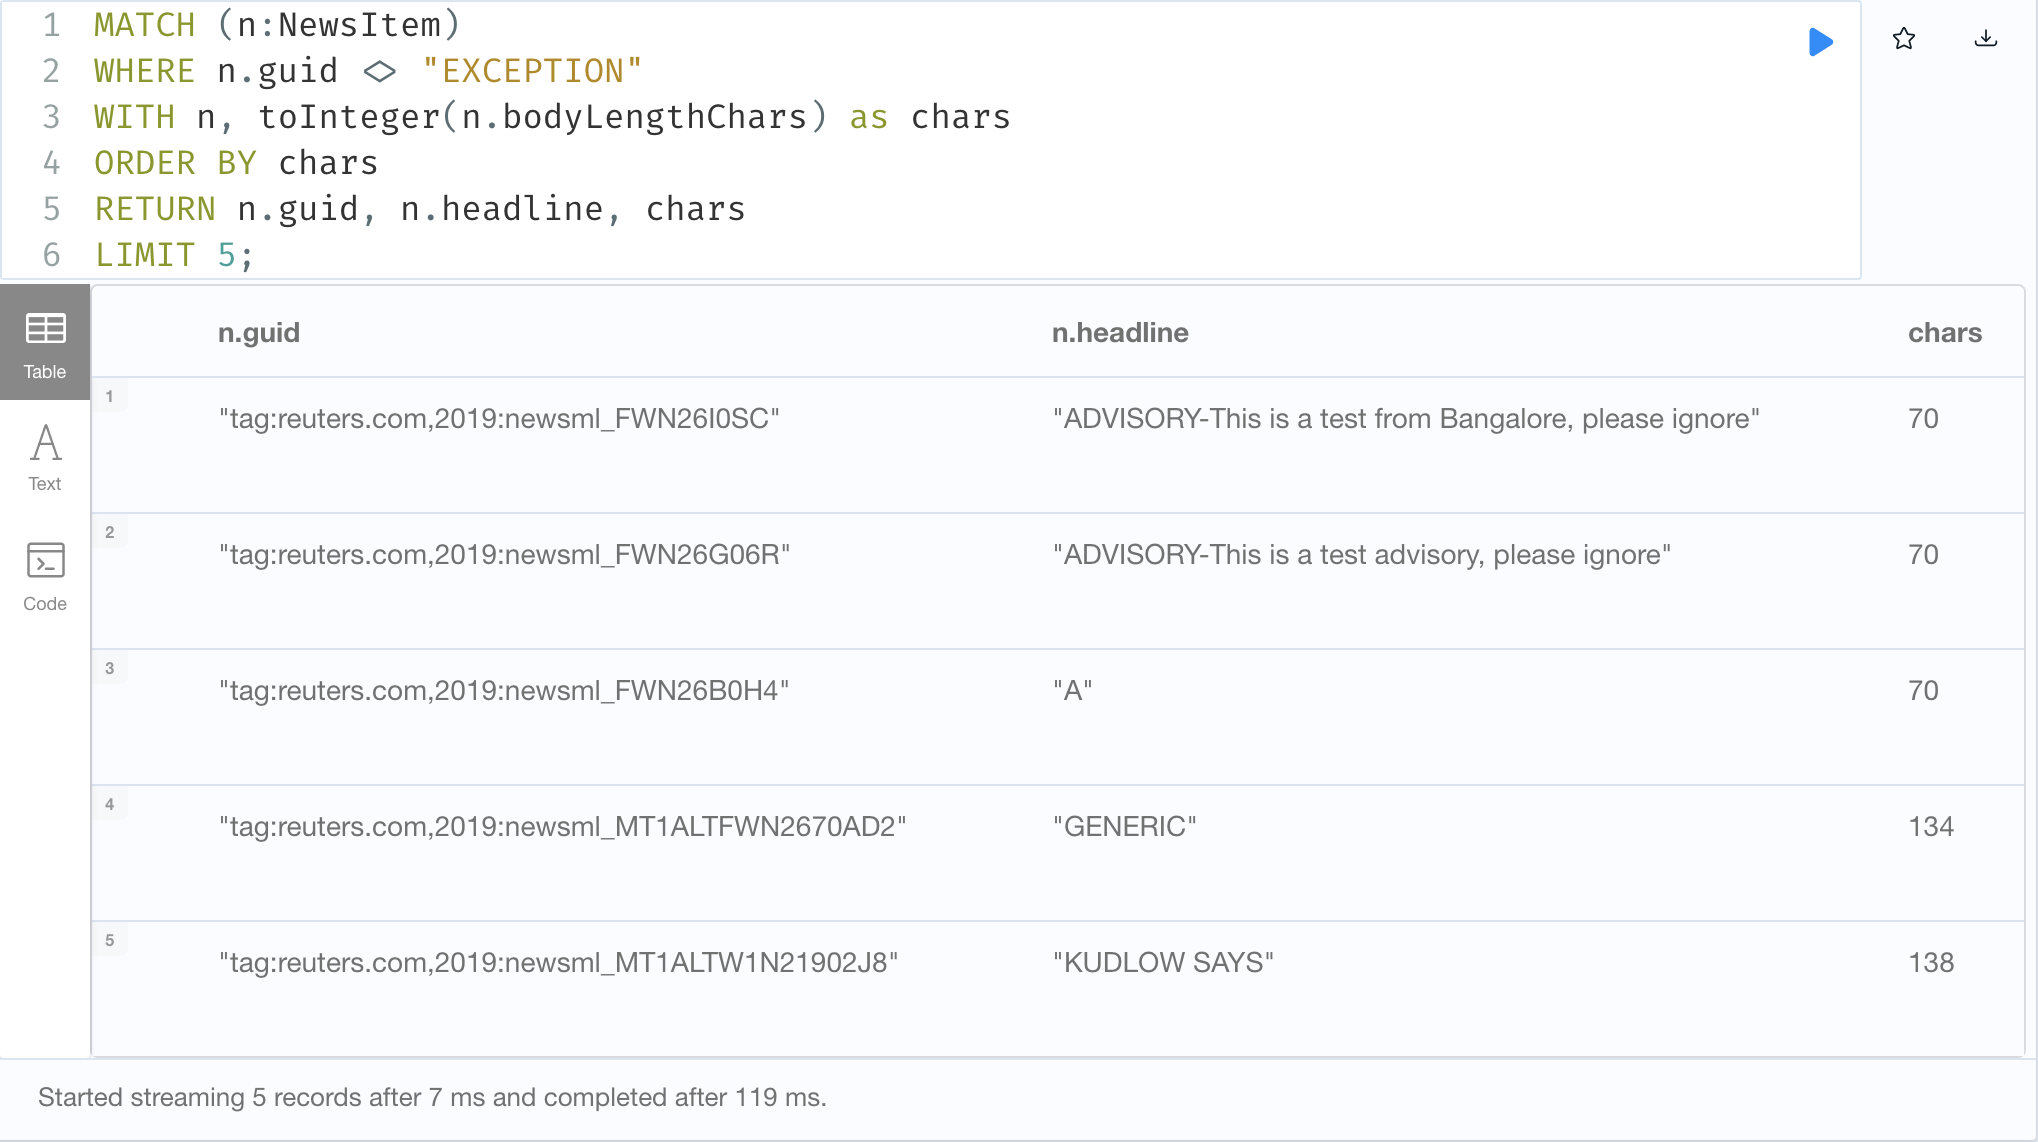
\includegraphics[scale=0.2]{01-shortest-items}
  \caption{\textit{Knowledge graph Cypher queries: shortest and longest news text}}
\end{figure}

\begin{figure}
  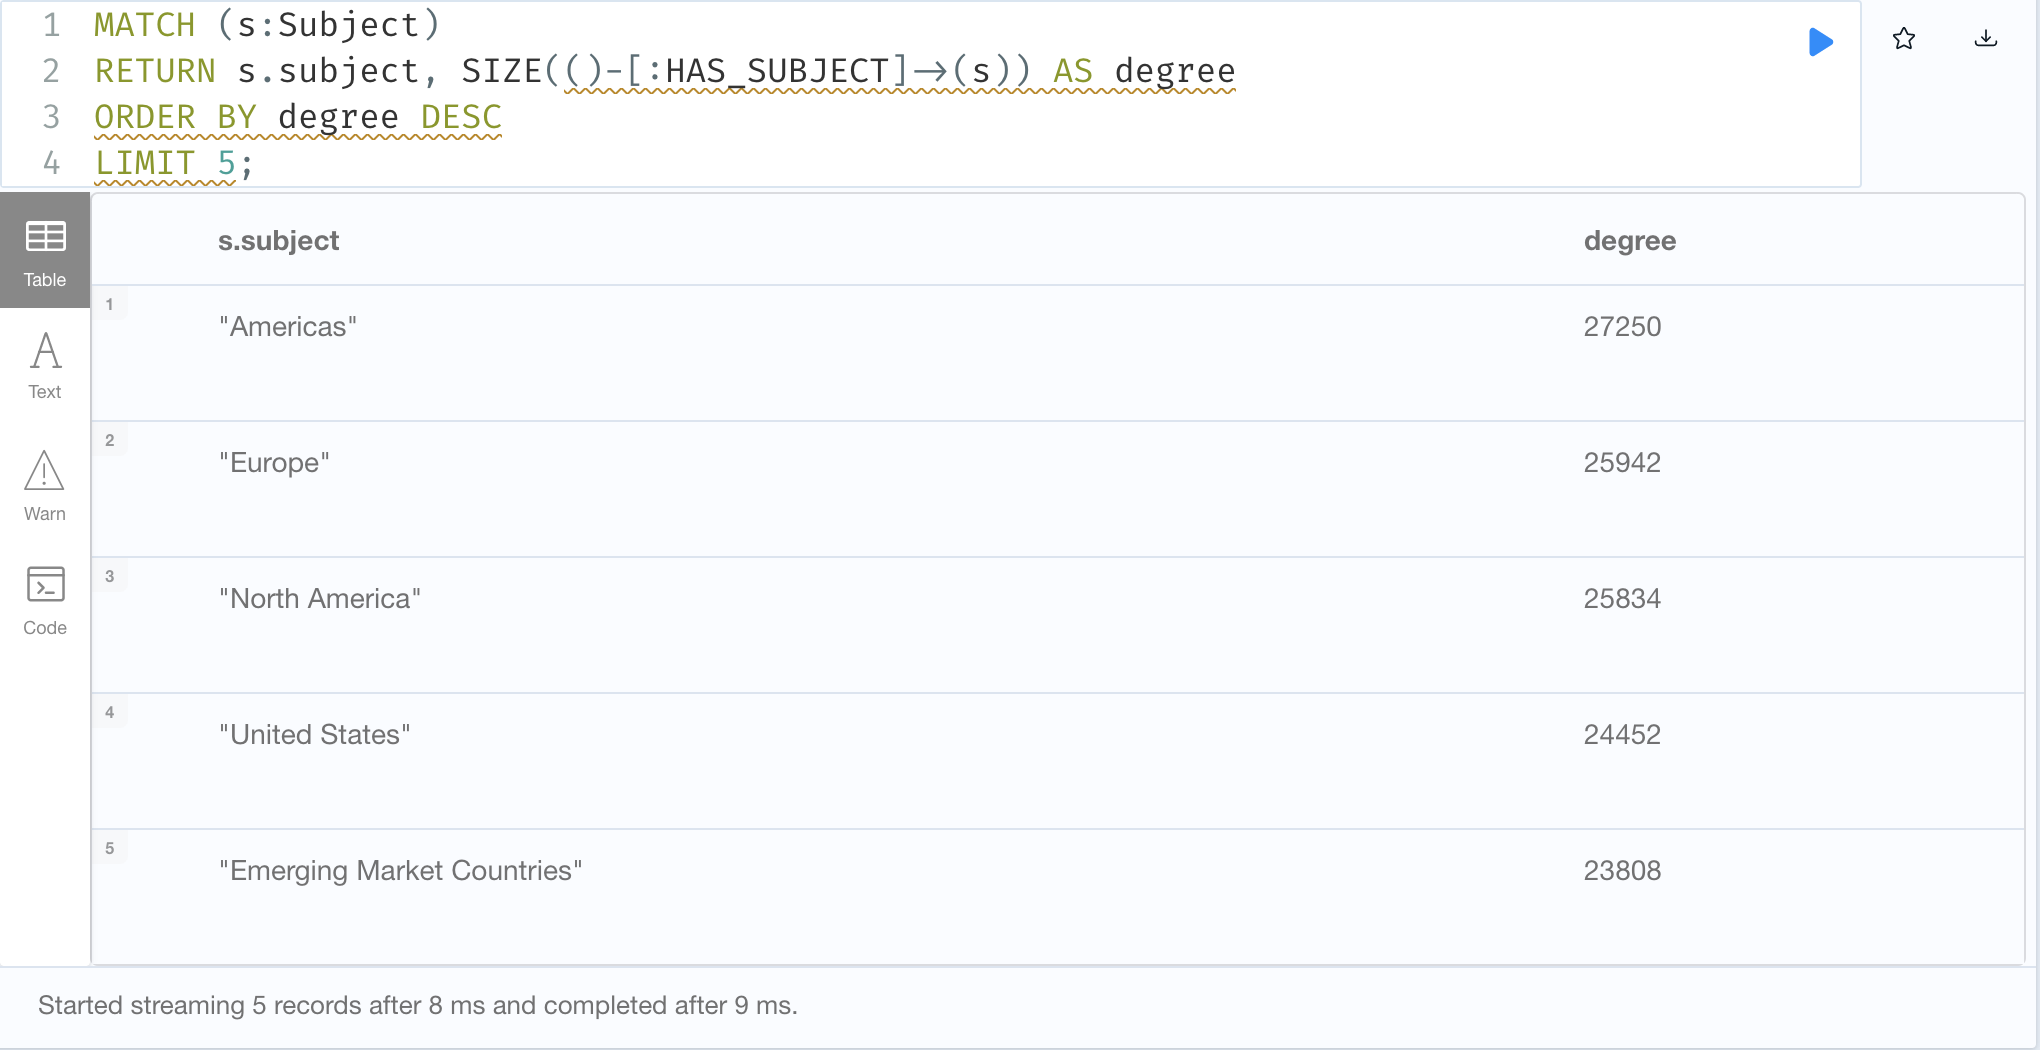
\includegraphics[scale=0.2]{02-subjects-with-most-items}
  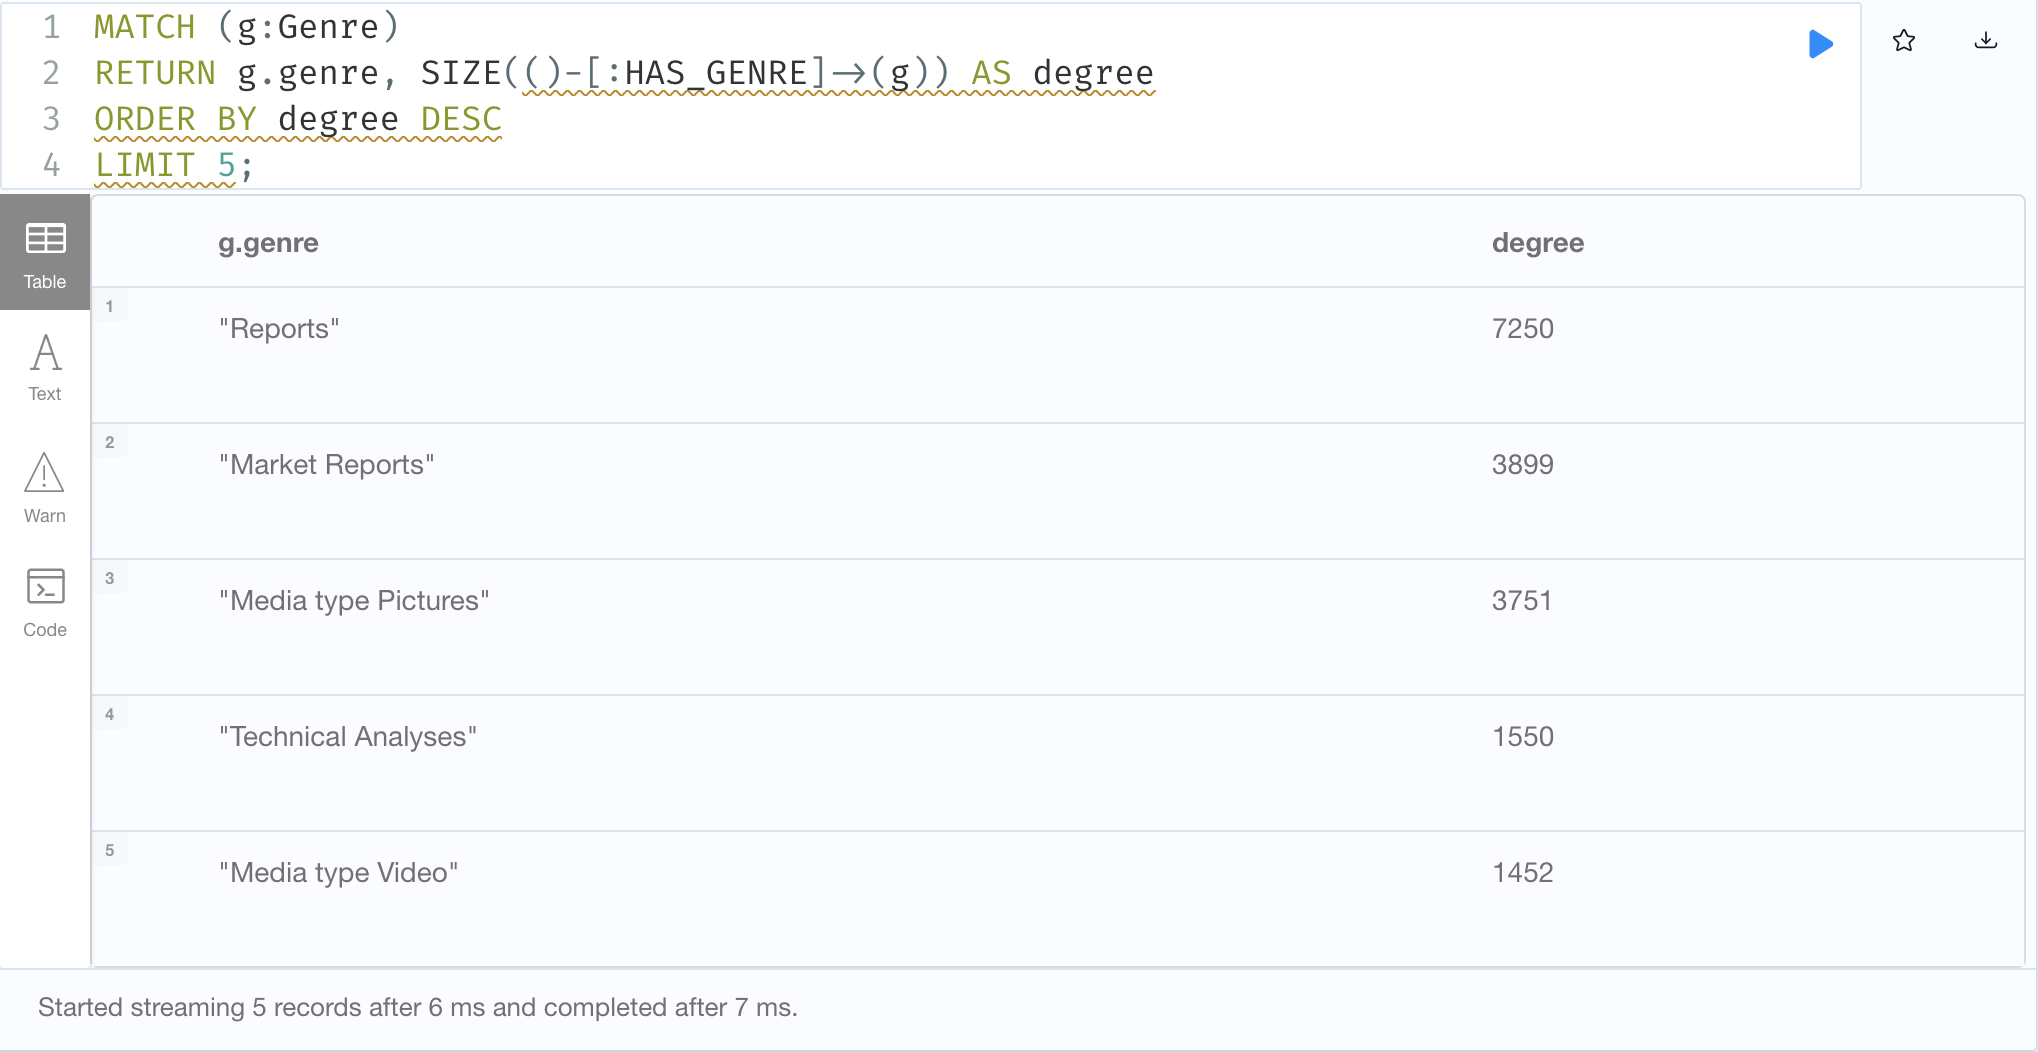
\includegraphics[scale=0.2]{02-genres-with-most-items}
  \caption{\textit{Knowledge graph Cypher queries: subjects and genres with most items}}
\end{figure}

\begin{figure}
  \centerline{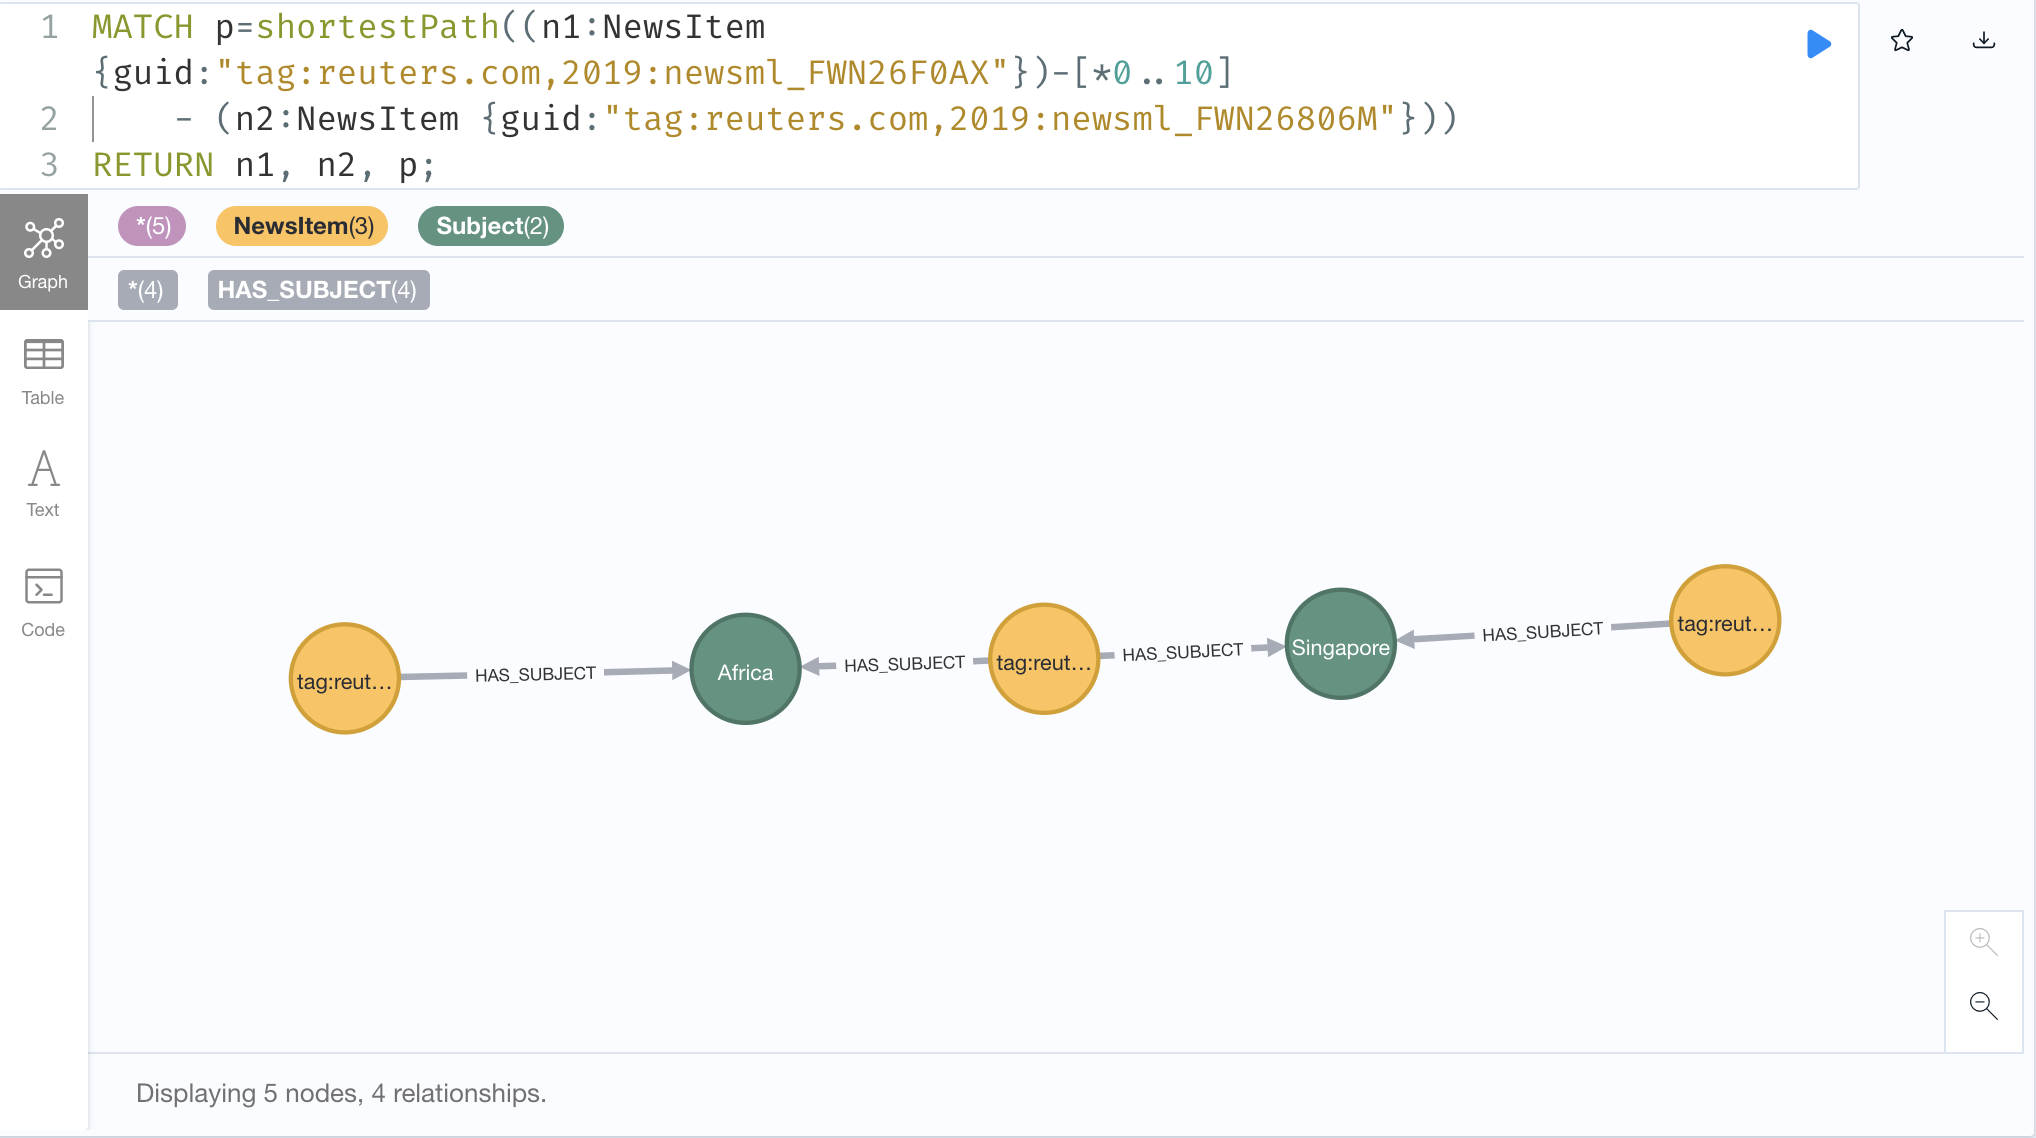
\includegraphics[scale=0.2]{03-shortest-path}}
  \caption{\textit{Knowledge graph Cypher queries: shortest-path}}
\end{figure}


\section{Knowledge Graph Design and Enhancement}

Building on the domain-sepcific knowledge graph of news items from the previous sections, the analysis now focuses on enhancements to the knowledge graph. This includes (1) semantic enhancements using ontologies and linked data; (2) NLP enhancements to extract entities and other meaning from the English language text; and (3) network analysies around centrality, clustering, and betweenness. 

\subsection{Semantic Enhancements}

RDF, wikidata

\subsection{Natural Language Processing}

Entity extraction

\subsection{Models, networks, etc.???}

Clustering, betweenness

\section{Knowledge Graph performance evaluation}

see evaluation.md

\subsection{Interpretability}
\subsection{Others...confusion matrix, predictions, clustering, betweenness, etc.}

\section{Conclusions}
\subsection{Future Work}
\subsection{Conclusion}


\newpage

\section{Appendix}
\subsection{Appendix XML...}
\label{sec:AppendixXML}
Sample XML document from Reuters corpus on AWS S3, specifically file \lstinline{tag/reuters.com,2019/newsml_L2N25V1DP/702697965}:
\\


\begin{lstlisting}
<?xml version="1.0" encoding="UTF-8"?>
<!-- 
SUMMARY: 
- Structure: NML2 SNI Text 
- Based On: NML2 v2.10

AUTHOR: thomsonreuters.com
-->
<!-- ========================================================= -->
<newsMessage xmlns="http://iptc.org/std/nar/2006-10-01/" xmlns:rtr="http://www.reuters.com/ns/2003/08/content" xmlns:x="http://www.w3.org/1999/xhtml" xmlns:xsi="http://www.w3.org/2001/XMLSchema-instance">
  <header>
    <sent>2019-09-04T20:08:51.000Z</sent>
    <sender>reuters.com</sender>
    <transmitId>tag:reuters.com,2019:newsml_L2N25V1DP:702697965</transmitId>
    <priority>3</priority>
  </header>
  <itemSet>
    <newsItem conformance="power" guid="tag:reuters.com,2019:newsml_L2N25V1DP" standard="NewsML-G2" standardversion="2.10" version="702697965" xml:lang="en">
      <catalogRef href="http://www.iptc.org/std/catalog/catalog.IPTC-G2-Standards_3.xml"/>
      <rightsInfo>
        <copyrightHolder literal="Thomson Reuters"/>
        <copyrightNotice xml:lang="en">(c) Copyright Thomson Reuters 2019. Click For Restrictions - https://agency.reuters.com/en/copyright.html</copyrightNotice>
      </rightsInfo>
      <itemMeta>
        <itemClass qcode="icls:text" rtr:msgType="S"/>
        <provider literal="reuters.com"/>
        <versionCreated>2019-09-04T20:08:51.000Z</versionCreated>
        <firstCreated>2019-09-04T20:08:51.000Z</firstCreated>
        <pubStatus qcode="stat:usable"/>
        <role qcode="itemRole:N"/>
        <fileName>2019-09-04T200851Z_702697965_L2N25V1DP_RTRMADT_0_EXXON-MOBIL-CHEVRON-BREAKINGVIEWS.XML</fileName>
        <generator versioninfo="1.0.0.21">LYNX:addT:001</generator>
        <profile versioninfo="00.00.01">SNI-Text</profile>
        <service qcode="svc:RTR_TNS"/>
        <instanceOf qcode="NI:CURRIE/"/>
        <signal qcode="edStat:N"/>
        <rtr:versionedId guid="tag:reuters.com,2019:newsml_L2N25V1DP:702697965"/>
      </itemMeta>
      <contentMeta>
        <urgency>3</urgency>
        <infoSource literal="Reuters" qcode="NS:RTRS" role="cRole:origProv"/>
        <creator literal="Reuters"/>
        <altId rtr:isOriginal="1" type="idType:EAID">23b9e59f-48cf-e911-718c-215056936dab</altId>
        <language tag="en"/>
        <subject qcode="N2:US" type="cptType:5">
          <name>United States</name>
          <facet qcode="geoProp:5"/>
        </subject>
        <subject qcode="N2:NAMER" type="cptType:5">
          <name>North America</name>
          <facet qcode="geoProp:3"/>
        </subject>
        <genre qcode="N2:BRV">
          <name>Reuters Breakingviews</name>
        </genre>
        <slugline separator="-">EXXON MOBIL-CHEVRON/BREAKINGVIEWS</slugline>
        <headline>BREAKINGVIEWS-Exxon CEO risks fueling unholy investor alliance</headline>
        <creditline>Reuters</creditline>
        <description role="descRole:caption">EXXON MOBIL-CHEVRON/BREAKINGVIEWS:BREAKINGVIEWS-Exxon CEO risks fueling unholy investor alliance</description>
        <by>By Antony Currie</by>
      </contentMeta>
      <assert qcode="R:XOM.N">
        <name>Exxon Mobil Corp</name>
        <sameAs qcode="NDAID:36999"/>
        <organisationDetails>
          <rtr:companydata exchange="NYS" exchangecv="MDNA" name="Exxon Mobil Corp" ric="XOM.N" tickersymbol="XOM"/>
        </organisationDetails>
      </assert>
      <contentSet>
        <inlineXML contenttype="application/xhtml+html" wordcount="209">
          <html xmlns="http://www.w3.org/1999/xhtml">
            <head>
              <title/>
            </head>
            <body>
              <p>(The author is a Reuters Breakingviews columnist.  The opinions
expressed are his own.)</p>
              <p>By Antony Currie</p>
              <p>NEW YORK, Sept 4 (Reuters Breakingviews) - Darren Woods
reckons human progress and the unreliability of alternative
energy sources justifies investing more in emissions-laden
fossil fuels. But his argument ignores the $293 bln driller's
poor returns. That may give financial investors common cause
with climate activists...</p>
            </body>
          </html>
        </inlineXML>
      </contentSet>
    </newsItem>
  </itemSet>
</newsMessage>
\end{lstlisting}
\newpage

\subsection{Appendix A. \textit{\lstinline{item_xml_docs_to_csv.py}} to transform XML docs to CSV}
\label{sec:AppendixA}
Save the following code as \textit{\lstinline{item_xml_docs_to_csv.py}} and run using command line arguments below with a directory of XML / NewsMLG2 documents.
\\

\begin{lstlisting}[language=Python]
% \begin{lstlisting}
import csv
import os
import re
import sys
import xml.etree.ElementTree as ET


NSMAP = {'iptc': 'http://iptc.org/std/nar/2006-10-01/',
         'xhtml': 'http://www.w3.org/1999/xhtml'}
CSV_ROW_LIMIT = 10000
VERBOSE = False

# workaround solution for encoded emojis in tweets
% INVALID_CHAR_REGEX = '&#\d\d\d\d\d;'

def save_to_csv(news_items, filename):
  fields = ['filename',
            'datetime',
            'guid',
            'slugline',
            'headline',
            'description',
            'genres',
            'subjects',
            'bodyLengthChars',
            'bodyLengthCharsNonWhitespace',
            'bodyLengthWords',
            # 'body'
            ]

  with open(filename, 'w') as csvfile:
    writer = csv.DictWriter(csvfile, fieldnames=fields)
    writer.writeheader()
    writer.writerows(news_items)

def make_news_item_dict(filename, body='', datetime='EXCEPTION', description='EXCEPTION',
                        genres='EXCEPTION', guid='EXCEPTION', headline='EXCEPTION',
                        slugline='EXCEPTION', subjects='EXCEPTION'):
  """
  Return dictionary of news_item. For empty case (in exceptions), default arguments
  will be 'EXCEPTION' and 0 length for bodyLengthChards and bodyLengthWords.
  """
  return {#'body': body,
          'datetime': datetime,
          'description': description,
          'filename': filename,
          'genres': genres,
          'guid': guid,
          'headline': headline,
          'slugline': slugline,
          'subjects': subjects,
          'bodyLengthChars': len(body),
          'bodyLengthCharsNonWhitespace': len(body.replace(' ', '')),
          'bodyLengthWords': len(re.split('\s+', body))} # split on \s+ for one *or more* spaces

def parse_xml(path, filename):
  file = path + '/' + filename
  try:
    root = ET.parse(file).getroot()
  except Exception as e:
    raise(e)
    with open(file, 'r') as file:
      data = file.read()
      data = re.sub(INVALID_CHAR_REGEX, '', data)
      root = ET.fromstring(data)

  guid = root.find('./iptc:itemSet/iptc:newsItem', namespaces=NSMAP).get('guid')

  subject_nodes = root.findall('./iptc:itemSet/iptc:newsItem/iptc:contentMeta/iptc:subject/iptc:name',\
                               namespaces=NSMAP)
  subjects = set()
  if len(subject_nodes) == 0:
    subjects = None
  else:
    for s in subject_nodes:
      subjects.add(s.text)

  genre_nodes = root.findall('./iptc:itemSet/iptc:newsItem/iptc:contentMeta/iptc:genre/iptc:name',\
                             namespaces=NSMAP)
  if len(genre_nodes) == 0:
    genres = None
  else:
    genres = set()
    for g in genre_nodes:
      genres.add(g.text)

  datetime = root.find('./iptc:itemSet/iptc:newsItem/iptc:itemMeta/iptc:firstCreated', namespaces=NSMAP).text
  slugline = root.find('./iptc:itemSet/iptc:newsItem/iptc:contentMeta/iptc:slugline',\
                       namespaces=NSMAP).text
  headline = root.find('./iptc:itemSet/iptc:newsItem/iptc:contentMeta/iptc:headline',\
                       namespaces=NSMAP).text
  description = root.find('./iptc:itemSet/iptc:newsItem/iptc:contentMeta/iptc:description',\
                          namespaces=NSMAP).text
  body = root.find('./iptc:itemSet/iptc:newsItem/iptc:contentSet/iptc:inlineXML/xhtml:html/xhtml:body',\
                   namespaces=NSMAP)#.text
  body = str(ET.tostring(body))

  return make_news_item_dict(filename, body, datetime, description, genres, guid,\
                             headline, slugline, subjects)

def parse_xml_and_write_csv(path, files, output_filename):
  counter = 0
  news_items = []
  n_files = len(files)
  check_length = n_files // 10 + 1
  for i, filename in enumerate(files):
    if VERBOSE:
      if i%check_length == 0:
        print(str(int(i/n_files*100)) + '% of this segment complete - Parsing file ' + str(i) + \
              ' out of ' + str(n_files) + ' - ', datetime.datetime.now())

    try:
      news_item = parse_xml(path, filename)
    except Exception as e:
      if VERBOSE: print('EXCEPTION: ', e, 'on file ', filename)
      news_item = make_news_item_dict(filename)
    news_items.append(news_item)

  if VERBOSE:
    print('Parsed next ' + str(n_files) + ' files')
    print('Saving to ' + output_filename + '...')

  save_to_csv(news_items, output_filename)

  if VERBOSE: print('Saved to ' + output_filename)

def parse_n_files(path='./', max_files=100000):
  files = os.listdir(path)
  files.sort()
  n_files = min(len(files), max_files)
  n_remaining_files = n_files

  if 'start_file_index' not in locals():
    start_file_index = 0
    end_file_index = start_file_index + CSV_ROW_LIMIT

  if VERBOSE:
    print('Parsing all ' + str(n_files) + 'XML files in directory')
    print()

  while end_file_index < n_files:
    end_file_index = start_file_index + CSV_ROW_LIMIT
    n_rows_in_csv = min(n_remaining_files, CSV_ROW_LIMIT)
    output_filename = 'output_' + str(start_file_index+1) + '_' + str(start_file_index + n_rows_in_csv) + '.csv'
    if VERBOSE: print('Parsing ' + str(n_rows_in_csv) + ' files into CSV rows in: ' + output_filename)
    parse_xml_and_write_csv(path, files[start_file_index:end_file_index], output_filename)
    n_remaining_files = n_remaining_files - n_rows_in_csv
    if VERBOSE:
      print('Completed parsing and saving of ' + str(n_files - n_remaining_files) + '/' + \
            str(n_files) + ' files (' + str((n_files - n_remaining_files) / n_files * 100) + '%)')
      print()
    start_file_index += CSV_ROW_LIMIT

# command line API
#   call with no params (from directory with XML files)
#       python item_xml_docs_to_csv.py
#   call with first arg as `path` param:
#       python item_xml_docs_to_csv.py ./text_en_201909
#   call with first arg `path` and second arg `max_files` param:
#       python item_xml_docs_to_csv.py ./text_en_201909 20
if __name__ == '__main__':
  if VERBOSE: print(datetime.datetime.now())
  if len(sys.argv) == 1:
    parse_n_files()
  elif len(sys.argv) == 2:
    parse_n_files(sys.argv[1])
  else:
    parse_n_files(sys.argv[1], int(sys.argv[2]))
  if VERBOSE: print(datetime.datetime.now())

\end{lstlisting}
\newpage

\subsection{Code to turn CSVs into Neo4j knowledge graph}
\label{sec:AppendixB}

\begin{lstlisting}
data-dimensions.ipynb...

\end{lstlisting}
\newpage


\subsection{Code to turn CSVs into Neo4j knowledge graph}
\label{sec:AppendixC}
\begin{lstlisting}
// after outputting reuters.csv, put it in Neo4j /import directory
// also put genres.csv, reuters.csv, and subjects-with-wikidata.csv
// in /import directory

// create 59k NewsItem nodes, one for each reuters item
CALL apoc.load.csv('/reuters.csv') yield map as row
CREATE (n:NewsItem) SET n = row;

CALL apoc.load.csv('/genres.csv') yield map
CREATE (g:Genre {genre: map.genre});

MATCH (g:Genre)
WITH g.genre AS genres
UNWIND genres AS genre
MATCH (n:NewsItem),(g:Genre)
WHERE n.genres CONTAINS genre AND g.genre = genre
CREATE (n)-[r:HAS_GENRE]->(g);

MATCH (n:NewsItem)-[r:HAS_GENRE]->(g:Genre)
RETURN n, r, g LIMIT 20;

CALL apoc.load.csv('subjects-with-wikidata.csv') YIELD map
CREATE (s:Subject) SET s = map;

MATCH (s:Subject)
WITH s.subject AS subjects
UNWIND subjects AS subject
MATCH (n:NewsItem),(s:Subject)
WHERE n.subjects CONTAINS subject AND s.subject = subject
CREATE (n)-[r:HAS_SUBJECT]->(s);

MATCH (n:NewsItem)-[r:HAS_SUBJECT]->(s:Subject)
RETURN n, r, s LIMIT 20;
\end{lstlisting}
\newpage


\subsection{Queries of knowledge graph...}
\label{sec:AppendixQuery}
\begin{lstlisting}
TBD...
\end{lstlisting}

\newpage
\bibliographystyle{abbrv}
\bibliography{project}

\end{document}